\documentclass{juliacon}

\setcounter{page}{1}

\usepackage{mathrsfs}
\usepackage{amssymb,amstext,amsfonts,amsmath}

\usepackage{todonotes}
\newcommand{\todoi}[2][]{\todo[inline,#1]{#2}}
\newcommand{\todoq}[2][]{\todo[inline,color=blue!20!white,#1]{#2}}

\usepackage{xspace}
\usepackage[labelformat=simple]{subfig}
\renewcommand{\thesubfigure}{(\alph{subfigure})}

\usepackage{calc}
\usepackage{graphicx,import}

\usepackage{comment}

% no number in references section
\usepackage[square,sort,comma,numbers]{natbib}

% algorithms-pseudocode
\usepackage{jlcode}
\usepackage{listings}

\lstset{
	language=Julia,
	basicstyle=\ttfamily\footnotesize,
	numberstyle=\scriptsize,
	backgroundcolor=\color{gray!10},
	frame=single,
	tabsize=2,
	rulecolor=\color{black!30},
	title=\lstname,
	escapeinside={\%(*}{*)},
	breaklines=true,
	breakatwhitespace=true,
	framextopmargin=2pt,
	framexbottommargin=2pt,
	extendedchars=true,
	inputencoding=utf8,
	columns=fullflexible,
}

% letters
\newcommand{\bfa}{{\bf a}}
\newcommand{\bfA}{{\bf A}}
%
\newcommand{\bfb}{{\bf b}}
\newcommand{\bfB}{{\bf B}}
%
\newcommand{\bfc}{{\bf c}}
\newcommand{\bfC}{{\bf C}}
%
\newcommand{\bfd}{{\bf d}}
\newcommand{\bfD}{{\bf D}}
%
\newcommand{\bfe}{{\bf e}}
\newcommand{\bfE}{{\bf E}}
%
\newcommand{\bff}{{\bf f}}
\newcommand{\bfF}{{\bf F}}
%g
\newcommand{\bfg}{{\bf g}}
\newcommand{\bfG}{{\bf G}}

\newcommand{\bfi}{{\bf i}}
\newcommand{\bfI}{{\bf I}}
%
\newcommand{\bfh}{{\bf h}}
\newcommand{\bfH}{{\bf H}}
%
\newcommand{\bfk}{{\bf k}}
\newcommand{\bfK}{{\bf K}}
%
\newcommand{\bfl}{{\bf l}}
\newcommand{\bfL}{{\bf L}}
% m
\newcommand{\bfm}{{\bf m}}
\newcommand{\bfM}{{\bf M}}
% n
\newcommand{\bfn}{{\bf n}}
\newcommand{\bfN}{{\bf N}}
% p
\newcommand{\bfp}{{\bf p}}
\newcommand{\bfP}{{\bf P}}
% q
\newcommand{\bfq}{{\bf q}}
\newcommand{\bfQ}{{\bf Q}}
% r
\newcommand{\bfr}{{\bf r}}
\newcommand{\bfR}{{\bf R}}
% s
\newcommand{\bfs}{{\bf s}}
\newcommand{\bfS}{{\bf S}}
% t
\newcommand{\bft}{{\bf t}}
\newcommand{\bfT}{{\bf T}}
% u
\newcommand{\bfu}{{\bf u}}
\newcommand{\bfU}{{\bf U}}
% v
\newcommand{\bfv}{{\bf v}}
\newcommand{\bfV}{{\bf V}}
%
\newcommand{\bfx}{{\bf x}}
\newcommand{\bfX}{{\bf X}}

\newcommand{\bfy}{{\bf y}}
\newcommand{\bfY}{{\bf Y}}

\newcommand{\bfw}{{\bf w}}
\newcommand{\bfW}{{\bf W}}

\newcommand{\bfz}{{\bf z}}
\newcommand{\bfZ}{{\bf Z}}

\newcommand{\bfvarep}{\boldsymbol{\varepsilon}}
\newcommand{\bfsig}{\boldsymbol{\sigma}}
\newcommand{\bfmu}{\boldsymbol{\mu}}
\newcommand{\bftau}{\boldsymbol{\tau}}
\newcommand{\bfPhi}{\boldsymbol{\Phi}}

% definitions reachability
\newcommand{\Reach}[3]{\mathcal{R}}
\def\mcX{\mathcal{X}}
\def\mcR{\mathcal{R}}
\def\mcU{\mathcal{U}}
\def\mcF{\mathcal{F}}

% rings and sets
\newcommand{\R}{\mathbb{R}}
                   
\begin{document}
	
% **************GENERATED FILE, DO NOT EDIT**************

\title{Computing Reachable Sets of Semi-Discrete Solid Dynamics Equations with ReachabilityAnalysis.jl}

\author[1]{Marcelo Forets}
\author[2]{Daniel Freire Caporale}
\author[3]{Jorge M. {P\'erez Zerpa}}
\affil[1]{Depto. de Matemática y Aplicaciones, CURE, UdelaR, Maldonado, Uruguay}
\affil[2]{Instituto de Física, Facultad de Ciencias, UdelaR, Montevideo, Uruguay}
\affil[3]{Instituto de Estructuras y Transporte, Facultad de Ingeniería, UdelaR, Montevideo, Uruguay}

\keywords{Reachability Analysis, Finite Element Method, Heat Transfer, Structural Dynamics, Numerical Verification}

\hypersetup{
pdftitle = {Computing Reachable Sets of Semi-Discrete Solid Dynamics Equations with ReachabilityAnalysis.jl},
pdfsubject = {JuliaCon 2019 Proceedings},
pdfauthor = {Marcelo Forets, Daniel Freire Caporale, Jorge M. {P\'erez Zerpa}},
pdfkeywords = {Reachability Analysis, Finite Element Method, Heat Transfer, Structural Dynamics, Numerical Verification},
}



\maketitle

\emph{The set-based approach.} %
%
Many real-world problems require the resolution of ODEs with uncertainties such as: initial conditions or applied loads. %
%
Obtaining solutions considering these uncertainties is a challenging task, particularly in large scale systems.
%
The set-based approach consists in the construction of sets that contain all the feasible solutions of the ODEs. %
% ---------------


\vspace{0.2cm}

\emph{Solid Dynamics ODEs.} %
%
In problems such as wave propagation or structural vibrations, solid dynamics problems are formulated. %
%
In these cases, large systems of ODEs of the form:
%
\begin{equation}\label{eq:second_order}
\mathbf{M} \mathbf{x}''(t) + \mathbf{C}\mathbf{x}'(t) + \mathbf{K}\mathbf{x}(t) = \mathbf{F}(t),
\end{equation}
%
are formulated using the Finite-Element Method (FEM)~\cite{Bathe2014}, where $\mathbf{x} \in \mathbb{R}^n$ is the displacements (or state) vector, and $\mathbf{M}$, $\mathbf{C}$ and $\mathbf{K}$ are the mass, damping and stiffness matrices, respectively. Depending on the problem $n$ is typically  between $10^2$ and $10^5$.

	
\vspace{0.2cm}

\emph{Set-based Solid dynamics.} %
%
When uncertainty is present in the initial conditions, the displacements and velocities can be considered in sets as: $\mathbf{x}(0) \in \mathcal{X}_0$ and $\mathbf{x}'(0) \in \mathcal{V}_0$. %
%
In \cite{forets2021combining} a novel approach for time integration of structural dynamics equations based on set-based techniques~\cite{althoff2020set} is presented. %
%
This approach allows to compute in a single integration the solution sets (or \emph{flowpipes}) that include all exact trajectories for uncertainties in initial conditions and applied loads. %
%


\vspace{0.2cm}


\emph{Set-based FEM implementation and application.} %
%
In order to apply the set-based approach for solid dynamics, the package \href{http://github.com/JuliaReach/ReachabilityAnalysis.jl}{ReachabilityAnalysis.jl}\cite{ReachabilityAnalysis} was extended, providing a simple interface that can also be connected with FEM analysis tools such as \href{http://onsas.org}{ONSAS}~\cite{onsas}.
%
The implementations developed can be used to solve large systems, however, in this abstract a minimal didactic problem is solved. %
%
A system of two masses loaded with a Heaviside step function as shown in Fig.~\ref{fig:diagram} is considered.
%

\begin{lstlisting}[label=ejemplo, numbers=left, aboveskip=-0.2cm, belowskip=0.8mm]
using ReachabilityAnalysis
m = 0.25; k = 2.0
M = [2m 0; 0 m]; K = [2k -k; -k k]; C = (M+K)/20
F = [0.0, 1.0]; ΔF0 = Interval(0.9, 1.1)
U0 = BallInf(zeros(4), 0.5)
sys = SecondOrderLinearContinuousSystem(M, C, K, F)
prob = InitialValueProblem(homogenize(sys), U0 × ΔF0)
solA = solve(prob, 50, LGG09(δ=5e-2, dirs=:box, dim=5))
solB = solve(prob, 50, LGG09(δ=5e-2, dirs=:oct, dim=5))
\end{lstlisting}

\begin{figure}[tb!]
	\centering
	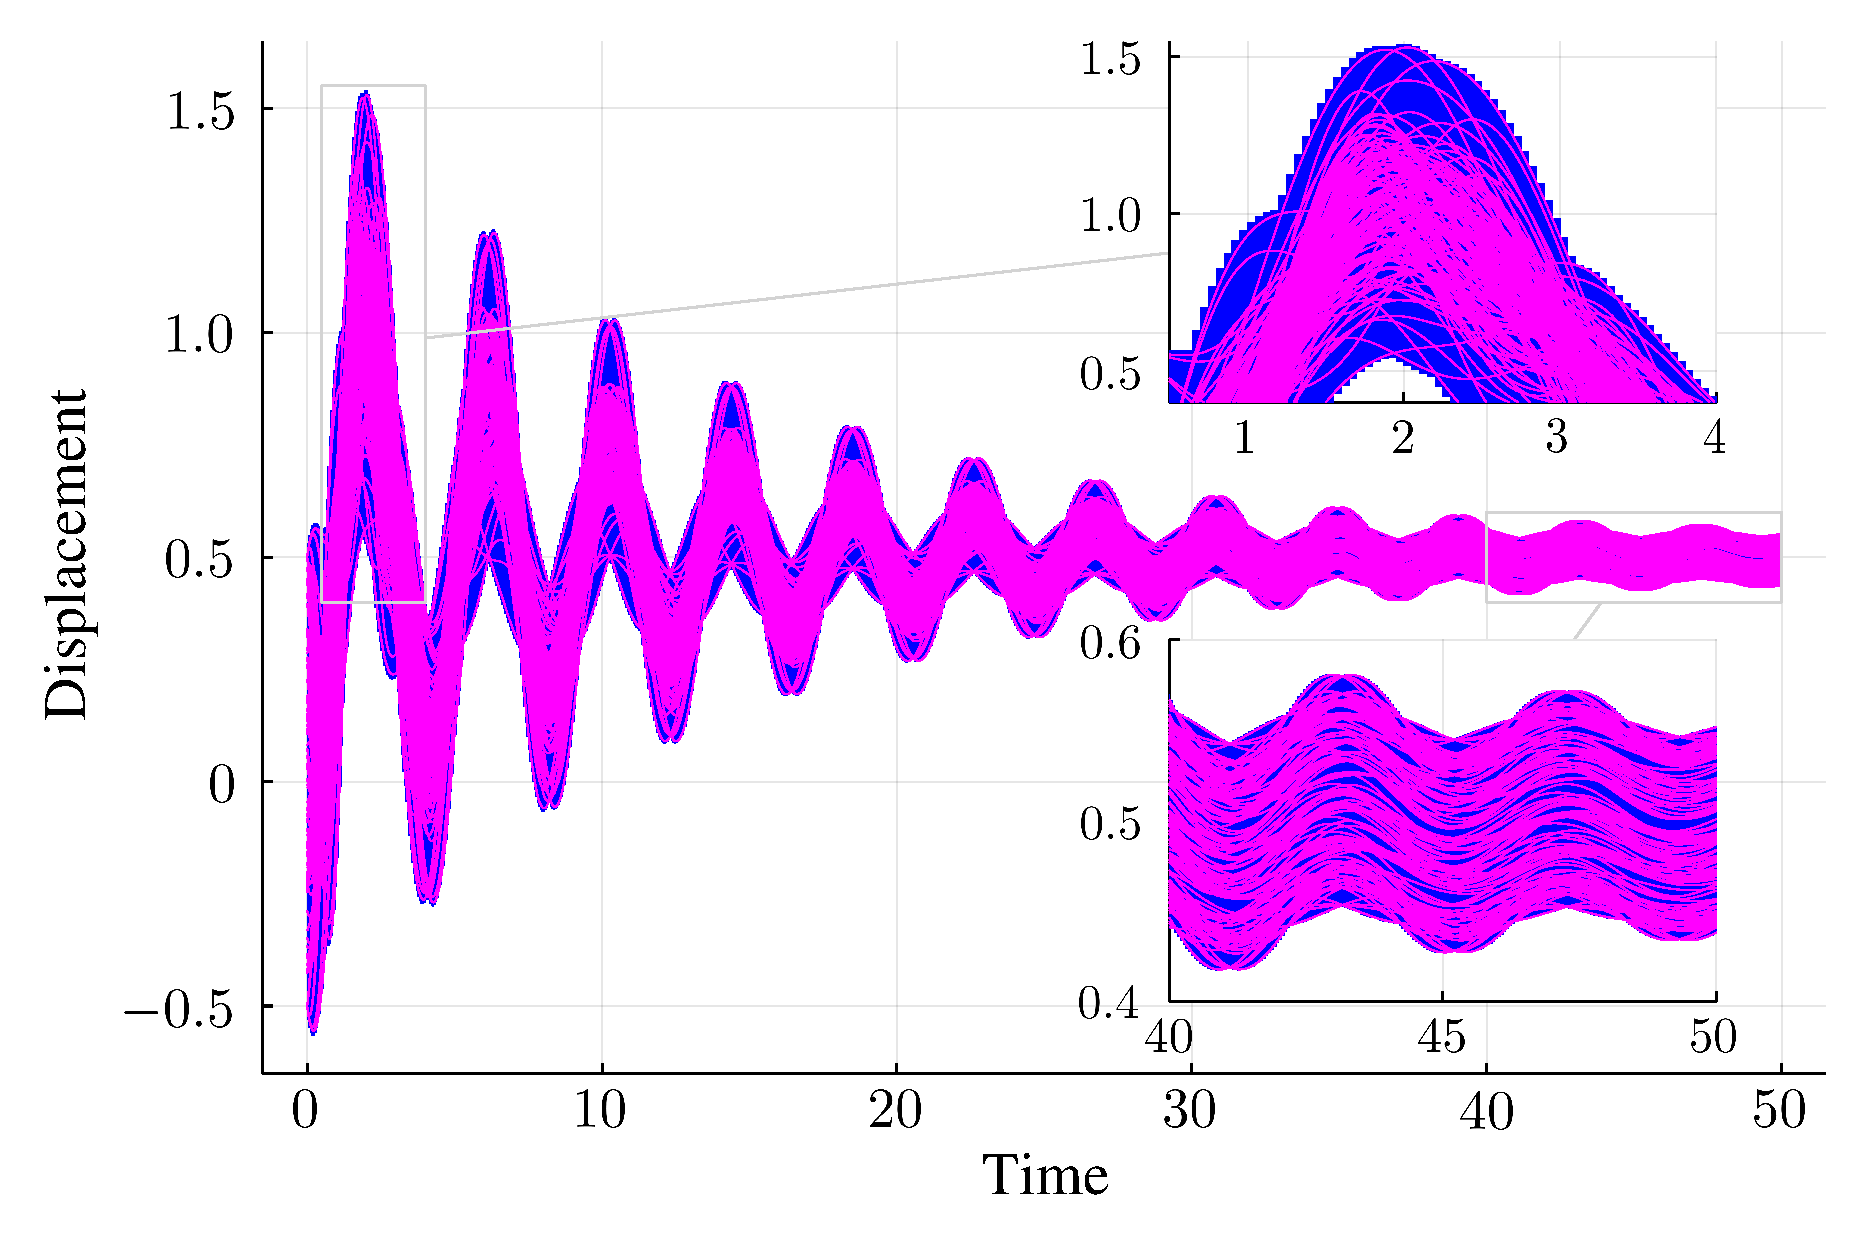
\includegraphics[width=0.8\linewidth,keepaspectratio]{example/displacement_vs_time}
	
	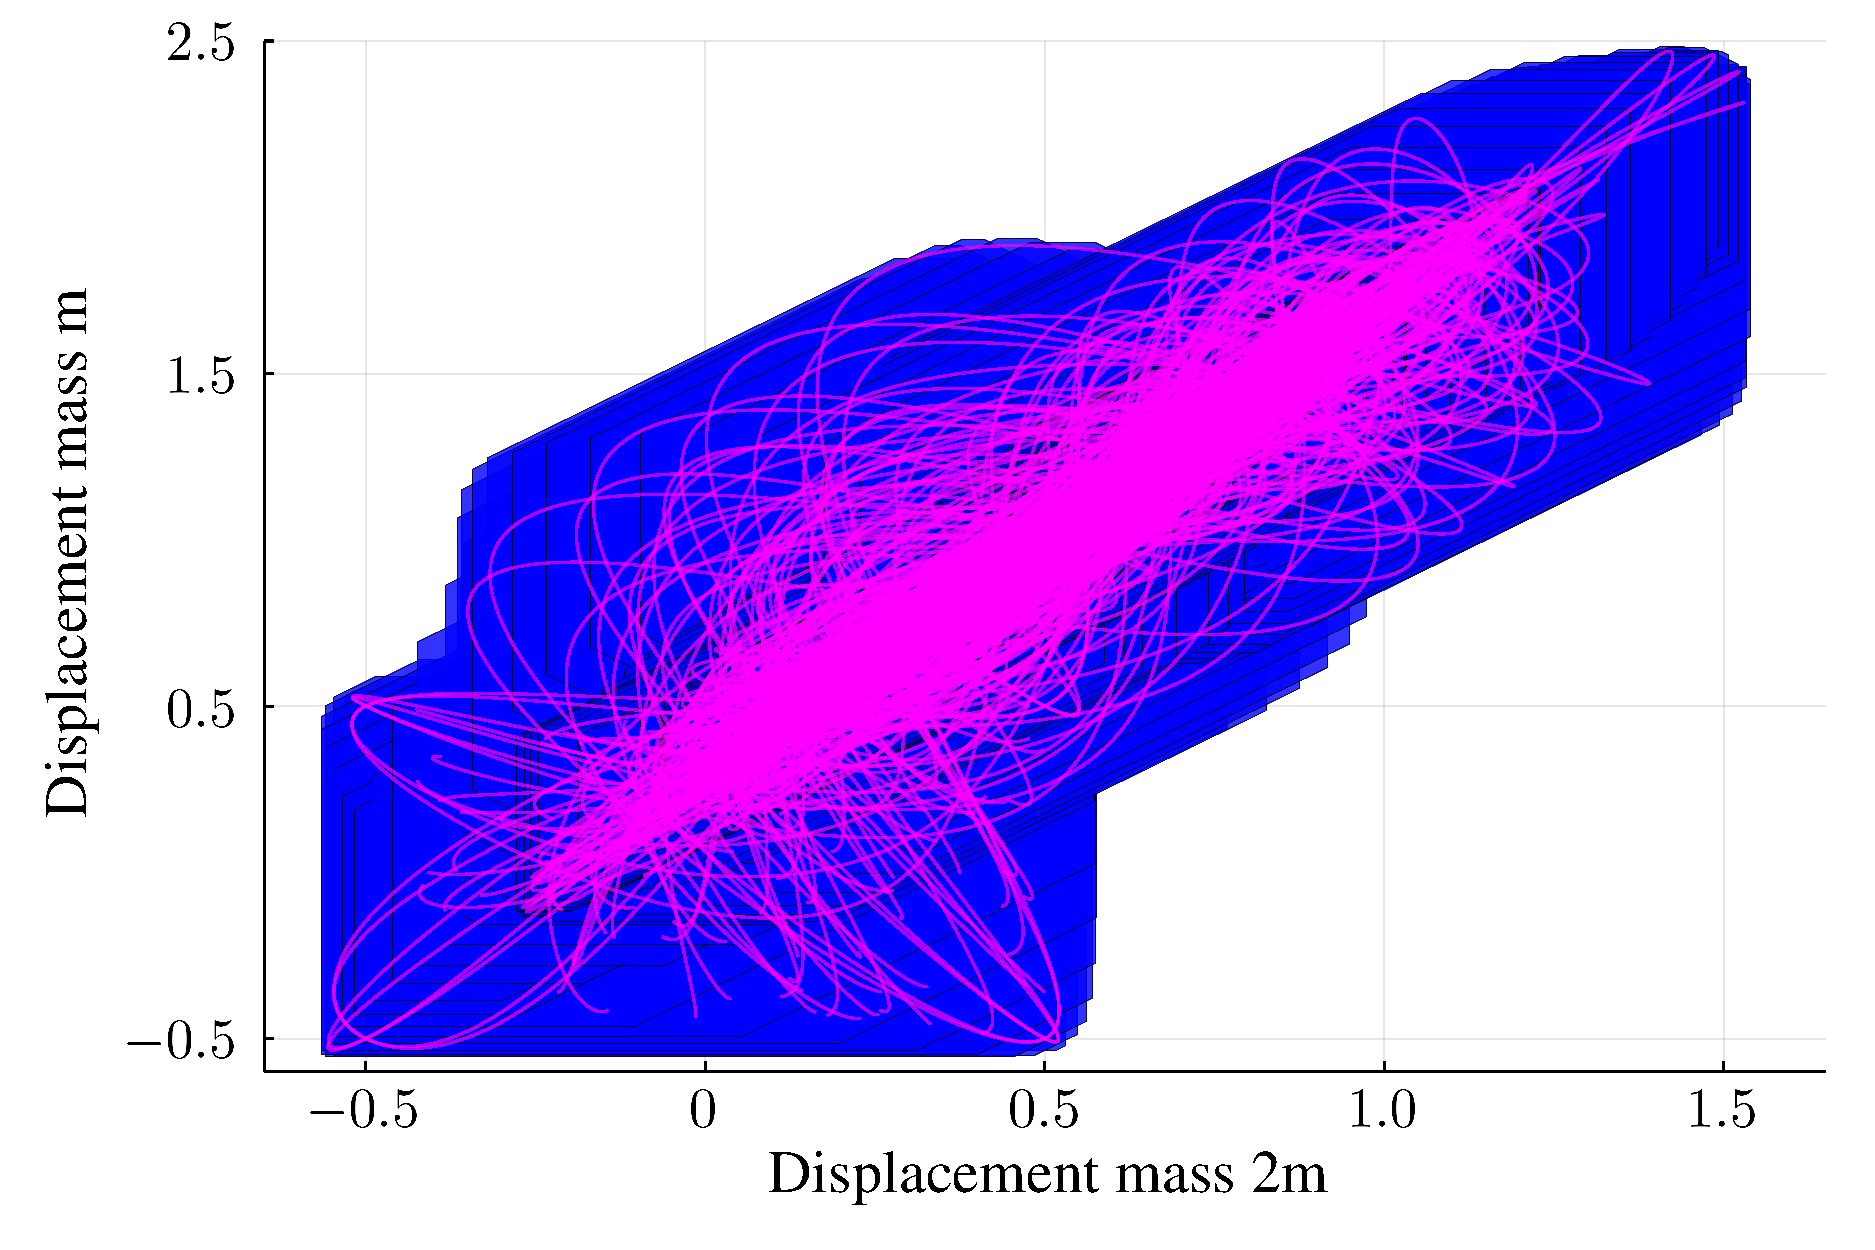
\includegraphics[width=0.8\linewidth,keepaspectratio]{example/displacement_vs_displacement}
	%
	\caption{Flowpipe of displacements of mass $2m$ projected on time computed using canonical directions  (top), and flowpipe of displacements computed using octagonal directions (bottom). We additionally plot random simulations.}
	\label{fig:example}
\end{figure}



\vspace{-0.1cm}

\begin{figure}[htb]
	\centering
 \def\svgwidth{0.25\textwidth}
 \input{diagram.pdf_tex}
 \caption{Diagram of two degrees of freedom and Rayleigh damping.}
 \label{fig:diagram}
\end{figure}


\noindent \emph{Solution method.} To illustrate the flexibility of our approach, two algorithm choices are considered, both relying on support functions~\cite{LeGuernic2010250} (\texttt{LGG09} algorithm in Lines 8-9).
%
\texttt{solA} contains the flowpipe efficiently computed along box directions $\pm e_1 = [\pm 1, 0, 0, 0]^T$, while \texttt{solB} contains the projection of the flowpipe for displacement coordinates of each mass. To improve the accuracy, the latter method uses octagonal template directions.

\vspace{0.2cm}

\noindent \emph{Perspectives.} We envision to model variations in mass and stiffness parameters using interval methods~\cite{forets2021intervalmat, ferranti2021interval}.
%
Probabilistic reachability, and modeling nonlinear behaviors using state-space abstraction methods, are also planned.
%
Julia has a thriving ecosystem of open source FEM projects~\cite{Gridap,Ferrite,FinEtools}, and we think that integrating set propagation into such tools is the next key step for solving real world problems using reachability.

\input{bib.tex}
	
\end{document}
